\documentclass[11pt,a4paper,twoside]{book}
%\usepackage{fullpage}
\usepackage[twoside,bindingoffset=0.6in,left=1in,right=1in]{geometry} %,left=1in,right=1in % margins
\usepackage{times}
\usepackage{pdfpages}
\usepackage[disable]{todonotes} % Todo
\usepackage[avantgarde]{quotchap} % Chapter headings
\usepackage{amsmath} % Math formatting 
\usepackage{amssymb} % "    "
\usepackage{setspace} % Spacing of the thesis
\usepackage{graphicx} % Includegraphics
\usepackage{algorithm2e} % Algorithms
\usepackage{graphpap}

\pdfimageresolution 300

\begin{document}
\frontmatter

\title{Thesis Results}
\author{Divye Kapoor}
\date{\today}
\maketitle

%\chapter{Candidate's Declaration}
\cleardoublepage
\addcontentsline{toc}{chapter}{Candidate's Declaration}
\includepdf{figures/candidate.pdf}

\chapter{Acknowledgements}

\onehalfspacing

I would like to take this opportunity to extend my most heartfelt gratitude to
my guide and mentor - \textbf{Prof. Manoj Misra}, Department of Electronics and
Computer Engineering, IIT Roorkee. His guidance, attention to detail and drive
for excellence have contributed greatly towards my education and also towards
ensuring that sterling work is done as part of my Masters dissertation. His
encouragement and unstinting faith have been essential in helping me learn, grow
and push the limits of my capabilities. I am fortunate to have been able to do
my dissertation under him.

My sincere thanks are due to \textbf{Dr. S. N. Sinha}, Professor and Head of the
Department of Electronics and Computer Engineering for providing the facilities
and hardware without which this thesis would have been all but impossible.
Thanks are also due to \textbf{Dr. Raheja}, Institute Architect, IIT Roorkee for
providing the blueprints of Ravindra Bhawan, the test site for this thesis. My
work would have been immensely more difficult without his help and cooperation.
The \textbf{Mahatma Gandhi Central Library} of IIT Roorkee also deserves a
mention in the Acknowledgements. They have provided unfettered access to the
world's highest quality research published in the IEEE and ACM journals. I have
always felt well supplied with information thanks to their hard work.

Sincere gratitude is also due to the authors of the many open source software
projects that have been very useful in the making of this thesis. The list of
projects is very long and it is impossible to name all, but I would like to give
a special mention to the authors and contributors of \textbf{\LaTeX, GNUPlot,
the GNU R Language, the GNU Core Utilities, Python, Linux, Android} and
\textbf{Eclipse}. This thesis is the result of standing on the shoulders of
giants and I am indebted to you for your efforts in maintaining such high
quality tools for the benefit of the world. Many many thanks.

Acknowledgements aren't complete without thanking \textbf{friends and family}.
They are the ones who have given unconditional encouragement and support. They
have shared my happiness on the days that things have worked and they have
helped get me through the days when things haven't. They have stood by me
through thick and thin and for that I am very grateful.



\chapter{Abstract}

The development of stable outdoor positioning and tracking algorithms has 
ushered in a new era of technology. Today GPS based navigators are 
ubiquitous and GPS based positioning and navigation has been integrated 
into smartphones. This has made life easy for navigation over large 
distances in an outdoor scenario. A new horizon for research has developed which
aims at providing that same ease of use in navigation 
and tracking in an indoor context.

Over the last few years, advances in technology have allowed for the 
development and integration of MEMS sensors into smartphones. These sensors 
(an accelerometer, a gyroscope and a magnetometer) can be leveraged to 
develop an indoor tracking solution. However, the resource constrained nature 
of smartphones necessitates modifications to prior work achieving the same 
in a non-mobile context. Additionally, the fact that 
the tracking device lies in a user's palm and not on a protected, stable 
surface (as is the case in robotics) generates a new set of challenges.

This thesis proposes and implements an online particle filter based algorithm for 
indoor positioning on an Android smartphone for pedestrians. The proposed algorithm 
is not only able to work well on the resource constrained device, it actually
yields an accuracy better than prior work in this area. Such results have 
been made possible by a careful approach to the problem with decisions made 
on factual data determined before and during the implementation of the 
proposed work. The final system is able to achieve a mean error of $0.5 m$
with a very low standard deviation value of $0.24 m$ and provides a clean,
intuitive tracked path. Results for comparison are produced using
a simple dead reckoning approach and a Nearest Neighbour 
Wifi corrected tracking algorithm. Both the algorithms are tested in the same
environment as the proposed work.



\tableofcontents
\clearpage

\listoffigures
\addcontentsline{toc}{chapter}{List of Figures}

\listoftables
\addcontentsline{toc}{chapter}{List of Tables}

\listofalgorithms
\addcontentsline{toc}{chapter}{List of Algorithms}

\clearpage
\listoftodos


\mainmatter

\onehalfspacing

\chapter{Introduction}

\section{Indoor Positioning}

Indoor positioning has been a topic of active research for the past decade with the first research system using RF signals for distance estimation and indoor positioning being produced by Microsoft Research (RADAR, 2000)\cite{RADAR}. Of course, systems like Active Badge  have been developed as far back as 1992 to locate targets indoors but they have shown limited utility on account of the requirement to deploy specialized sensors for detecting the radio tags deployed within the system.

Since RADAR, a number of improvements have been made in the core algorithms and technologies for positioning. Over time, indoor positioning has progressed from simply using RF signals to using ubiquitous 802.11 Access Points as radio sources. With the development of UWB (Ultra Wide Band) technology, very fine grained ranging and tracking results have been obtained over target distances of the order of a few hundred feet from the radio source. 

However, the primary scale of interest for commercial exploitation of indoor positioning and tracking is of the order of the size of warehouses and malls (~2500 m2 or more) with an accuracy that is preferably of the order of a few meters. The target applications for such a scenario are inventory location and tracking; location based services and personalized offers from businesses based on physical proximity to their shops or other points of sale. The ultimate target to be achieved in this line of research is:

Create a low complexity, low cost indoor positioning system that is maintainable, reasonably accurate and highly scalable.

UWB, unfortunately, does not scale easily to such large spaces without requiring that a significant number of sensors and repeaters be installed in the target positioning area specifically for this purpose. It is also an expensive technology. On the other hand, IEEE 802.11 AP based positioning has low complexity and cost and it has a large installed base, thus making it attractive for positioning purposes as a source of radio signals.

Thus it is interesting to explore the limitations of accuracy, scalability and maintainability of indoor positioning systems that are based on IEEE 802.11 Access Points.


\section{Indoor Tracking}

While exploring indoor positioning, another major application of such a system leaps out - Indoor Tracking. Indoor tracking refers to the process of tracking the location of a body on a continuous basis.


\section{Motivation}

  \subsection{Indoor Navigation}

  Describe indoor navigation applications (shops etc.)
  Why is it required?

  \subsubsection{Shipping industry}
  Courier delivery etc.


  \subsection{Augmented Reality}

  Describe AR.

  \subsubsection{Fusion Gaming}

  Describe potential applications to games in the real world.

  Describe AR, real-world games, indoor navigation, shopping complexes, warehouses.


\section{Problem Statement}
  Describe the problem to be solved.

\chapter{Literature Review\label{chap:literature_review}}

\section{Location! Location! Location!}

Knowing and finding where we are or where we should be is a very frequent 
task that is performed by us multiple times a day. We solve this problem 
in a variety of ways:

\begin{enumerate}
\item Use our prior knowledge and mental map of our surroundings
\item Ask around
\end{enumerate}

\section{Indoor Positioning}

Indoor positioning has been a topic of active research for the past decade with
the first research system using RF signals for distance estimation and indoor
positioning being produced by Microsoft Research (RADAR, 2000)\cite{RADAR}. Of
course, systems like Active Badge\cite{ActiveBadge} have been developed as far
back as 1992 to locate targets indoors but they have shown limited utility on
account of the requirement to deploy specialized sensors for detecting the radio
tags deployed within the system.

Since RADAR, a number of improvements have been made in the core algorithms and
technologies for positioning. Over time, indoor positioning has progressed from
simply using RF signals to using ubiquitous 802.11 Access Points as radio
sources. With the development of UWB (Ultra Wide Band) technology, very fine
grained ranging and tracking results have been obtained over target distances of
the order of a few hundred feet from the radio source. 

However, the primary scale of interest for commercial exploitation of indoor
positioning and tracking is of the order of the size of warehouses and malls
(approximately of the order of $2500 m^2$) with an accuracy that is preferably
of the order of a few meters. The target applications for such a scenario are
inventory location and tracking; location based services and personalized offers
from businesses based on physical proximity to their shops or other points of
sale. The ultimate target to be achieved in this line of research can be
paraphrased as:

\begin{quote}
Create a low complexity, low cost indoor positioning system that is
maintainable, reasonably accurate and highly scalable.
\end{quote}

UWB, unfortunately, does not scale easily to such large spaces without requiring
that a significant number of sensors and repeaters be installed in the target
positioning area specifically for this purpose. It is also an expensive
technology. On the other hand, IEEE 802.11 AP based positioning has low
complexity and cost and it has a large installed base, thus making it attractive
for positioning purposes as a source of radio signals.

Thus it is interesting to explore the limitations of accuracy, scalability and
maintainability of indoor positioning systems that are based on IEEE 802.11
Access Points.


\section{Indoor Tracking}

Once having worked with indoor positioning systems, it is but natural to ask:
Can we extend all the technology developed for indoor positioning to track 
objects and devices? Also, can we do it fast enough to provide a near-realtime
experience?

Research shows that the answer to both the questions is in the affirmative
and papers as far back as 2000 \cite{RADAR} have attempted to achieve this 


\section{Research gaps}



%\chapter{Problem Description}
To develop and evaluate a high accuracy tracking system on a modern smartphone using sensor fusion techniques.



\chapter{Proposed Method\label{chap:proposed_method}}
The particle filter approach described in [ped. Nav.] is adapted to and
implemented on the Android smartphone. The onboard accelerometer and
magnetometer of the Nexus S are used as inertial navigation sensors.
Improvements are made to the algorithm. The performance of the particle filter
is analyzed with different parameters and approaches:

\section{Dead reckoning with step counts}

The acceleration of the human body as part of the act of walking is small and 
very impulsive in nature. The motion of the torso of the body is governed 
mostly by inertia. Unfortunately, the impulsive acceleration values are small 
and lie buried in sensor noise. They are virtually indetectible using the MEMS 
accelerometer supplied with the android device - Nexus S.

To overcome this difficulty, the step count method of [ped. Nav.] is adopted. 
Under the assumption that step size varies very little over the course of 
motion of the subject, an inertial navigation system may be created.

\subsection{Step counting method}

The step counting method is described in [ped. Nav.]. However, we take a
slightly modified approach.  

\subsection{Noise clamping\label{sec:NoiseClamping}}

The MEMS accelerometer sensor on the smartphone has sensor noise present close
to zero. The noise level for the accelerometer was determined to be always less
than $0.6 m/s^2$. To allow for a reasonable noise margin and provide sufficient
cushion for additional noise introduced due to the dynamic nature of walking, we
choose a threshold of $1.3 m/s^2$. If the absolute value of the Z-axis
acceleration sample is less than this threshold, then the sample will be clamped
to zero. 

As has been determined experimentally, steps taken by a human usually produce
a pair of spikes - one positive and one negative with magnitude around $2 m/s^2$.
By choosing this threshold value, we give maximal noise margin for step detection.

See figure [...] for a comparative estimation of step values versus sensor noise.

\subsection{Step size detection procedure}

\subsubsection{Zero Crossings}

To detect actual steps taken by the subject holding the device, [ped. Nav.] 
suggests using zero crossings. However, in the sensor data collected, a number
of spurious zero crossings exist (primarily due to sensor noise). However, 
even after sensor noise is clamped as per section \ref{sec:NoiseClamping}, 
spurious zero crossings often arise due to variable motion of the subject.

\subsubsection{Peak and Valley hunting}
Peak and Valley hunting procedure (better than zero crossings) for step detection.
Robust to unexpected values.

To have robust detection of steps, a state machine is maintained. The state 
machine detects a peak and then waits for a trough. Subsequent

An internal state machine is used. The state machine has 2 states and a comparison
is made between $A_{max}$ or $A_{min}$ and the sample value that forms the peak/trough
whenever state transitions occur.

\begin{table}[h]\centering
    \caption{State table of the step detection state machine}
    \begin{tabular}{cccc} \hline
    State & Accelerometer Value     & New State &  Action\\     \hline
    $q_0$ & Positive Peak Detected  & $q_1$     & Update $A_{max}$ if peak is of larger magnitude \\
          & Other values            & $q_0$     & Ignore \\         \hline
    $q_1$ & Negative Trough Detected & $q_0$    & Update $A_{min}$ if trough is negative \\ 
          &                         &           & and of larger magnitude than $A_{min}$ \\
          & Other values            & $q_1$     & Ignore \\ \hline
    \end{tabular}
\end{table}
\subsection{Step Size Estimation}

Reference [A. Engineers] provides this empirical relationship between acceleration
values and step size.

\begin{equation}
 Step-size = C \sqrt[4]{A_{max} - A_{min}}
\end{equation}

The constant $C$ is a scaling factor that is used as a constant of proportionality
to scale the step-values to real world distances.

\section{Determining the Training Constant}
A simple procedure was followed to determine the training constant for a user.
The user was asked to locate himself using a QRCode before starting out along
a straight line along a corridoor

\section{Sensor fusion using Particle Filters}

A background on particle filters has already been given.

\subsection{Dynamical equations for system}

The dynamical equations that govern the system are:



\subsection{Accelerometer}


\subsection{Orientation}

\subsection{Camera info}
For first fix, we use QR codes. They are used whenever subject changes floors too.
The QR codes provide information about the map of the floor, the current location
and any additional information that is required by the tracking algorithm.

\subsection{Map Information}



\subsection{Wifi Information}

\section{Accounting for orientation bias and noise}

\section{Accounting for varying step sizes}

\section{Barometer Information}



\chapter{Implementation Details\label{chap:implementation_details}}

\section{Background on Android Application Development}

\subsection{The Android OS}

The Android OS was initiated as an open source project by Google  
to make application development easier for mobile devices. In order to 
do so, Google engineers created a customized Java Virtual Machine 
(called Dalvik VM) with resource saving features 
to make running Java applications on embedded devices feasible.
A large section of the Java Standard Library was then bolted onto the 
JVM by leveraging the open source Apache Harmony project.\todo{cite both} 
The typical structure of an Android Application built on the Android OS 
is shown in Figure \ref{fig:Android_OS_Structure}.

\begin{figure}
\centering
\includegraphics[width=4in]{figures/Android_OS.png}
\caption{Typical Structure of Android OS\label{fig:Android_OS_Structure}}
\end{figure}

\subsection{Application Development Tools}

Applications for Android are usually written in Java and are run on the 
custom Dalvik VM. Embedded programming is usually difficult because of 
limited visibility of the way the code runs on the target device (a smartphone).
To make development of apps for Android easier, custom tooling for Android 
has been developed that integrates with the Eclipse IDE toolchain.
The tools help to
interface with a development smartphone running an Android OS. They provide a
direct install-uninstall mechanism for applications under development 
and they also provide a debug bridge - called the ADB through which 
the Application code running on the smartphone may be debugged via debugging
tools on the host computer. A logging mechanism is also provided wherein 
application logs running on the device may be made visible in realtime 
on the host computer through the ADB. These tools go a long way in making 
development easier and help the programmer detect root causes of bugs faster.

\section{The Android Application Lifecycle\label{sec:android_lifecycle}}

Android applications are very different from the normal system executables
that we are used to programming. Executables once launched have complete 
system control during execution. They demand resources and release them at 
will depending on how they have been programmed. They are pre-empted and 
resumed transparently by the Kernel scheduler. However, such a mode of
execution is unsuitable for applications built for the mobile device. 
These applications need to be aware of their internal state at all times.
The user may pre-empt any application at any time and the system may 
suspend or even kill applications without warning to reclaim resources.
Applications are therefore expected to be written to follow an event machine 
lifecycle and are expected to save their state whenever they get pre-empted. 
The lifecycle of a typical Android application is shown in 
Figure \ref{fig:android_lifecycle}.


\begin{figure}
\centering
\includegraphics[height=5in]{figures/Android_lifecycle.png}
\caption{Android Application Lifecycle (Simplified)\label{fig:android_lifecycle}}
\end{figure}

The application typically starts off the 'Created' state, progresses 
to the 'Resumed' state. It may oscillate between the 'Resumed' and 'Paused' states
several times during the course of the execution lifetime of the application 
and then it finally transitions to the 'Finished' state when it is killed by 
the system either automatically or in response to a user action. All 
processing in the application is done either in response to a User action, 
a state change in the application lifecycle or in response to System 
messages delivered asynchronously to the application via \emph{BroadcastReceivers} 
or \emph{Intents}. (\emph{BroadcastReceiver} and \emph{Intent} are important
classes in the Android framework).

\subsection{Sensor Event Delivery Mechanism}

Sensor events are not delivered synchronously to the system in response to 
a function call as this would require a polling mode of operation which 
is a great drain on system resources - especially the battery. Instead, 
system events are delivered asynchronously to the application code 
in a thread created by the Android OS and which is owned by the 
Android Sensor Manager API. Thus any code written to handle sensor event 
delivery must be multithreaded aware and should be able to handle 
race conditions. The act of registering and unregistering for sensor events
with the Sensor Manager API still remains a synchronous operation though.
Figure \ref{fig:sensor_event} clarifies via a diagram the nature of the 
sensor event delivery mechanism and the synchronous and asynchronous operations
involved.

\begin{figure}
    \centering
    \includegraphics[width=5in]{figures/Android_Sensor_Setup.png}
    \caption{Synchronous and Asynchronous operations involved in registering for sensor events\label{fig:sensor_event}}
\end{figure}


\section{System Architecture}

As is clear from the previous section, the Android OS expects applications to 
be event-driven. In our case, events are being generated by the user 
not through direct interaction with the application via the UI but through 
indirect interaction via the sensors onboard the device. This naturally 
leads to a bottom-up design of the system on the lines similar to protocol
stacks seen commonly in the case of Computer Networks. The analogy
being drawn here is that a packet receive event in the case of a 
protocol stack is similar to a sensor event generated for our system. 

The complete layered structure of the application is shown in Figure 
\ref{fig:system_architecture}.

\begin{figure}
    \centering
    \includegraphics[width=5in]{figures/SysArch.png}
    \caption{System Architecture\label{fig:system_architecture}}
\end{figure}

At the bottom we have the \textbf{Sensor Unification Layer}. This layer is 
important as the Android API separates the event delivery mechanism 
for a Wifi SCAN event and the event delivery mechanism for a sensor 
sample event and a unification mechanism is thus required. 
The rationale behind the separation of concerns in the Android API is 
that sensors are passive environment samplers while the Wifi NIC is an active communication 
device and is not typically intended to be used as a sensor. The \textbf{Sensor 
Unification Layer} works very hard to unify Wifi {\tt SCAN\_RESULTS\_AVAILABLE} event results and 
sensor sample results into a single uniform events system to which 
a higher layer can subscribe by registering a callback object. Whenever 
a sensor event takes place for which higher layers have requested notification,
all registered callbacks for that event are executed by this layer. Thus,
higher layers can request access to sensor events by just registering an 
appropriate callback with this layer. The unification layer takes care of 
interfacing with the Android SensorManager API and the Android WifiManager API
and exposes lifecycle methods - \texttt{pause} and \texttt{resume} which free up 
higher layers from performing appropriate registrations and de-registrations
of sensor event handlers when they intend to go to sleep. The class that 
provides the API for the higher layers is the \emph{SensorLifecycleManager} class
and the critical class for implementation of this layer is the 
\emph{HWSensorEventListener} and \emph{WifiScanEventListener} classes. 

The layer immediately above the \textbf{Sensor Unification Layer} is the 
\textbf{Step Detection Layer}. This layer is responsible for accepting 
accelerometer and magnetometer sensor events from the device and notifying 
callbacks that a step event has taken place. The callbacks receive 
notification of the step event along with parameters which 
indicate the \texttt{step size}, the \texttt{step angle} and a 
\texttt{timestamp} of the event. 

The \textbf{Step Detection Layer} essentially feeds the \textbf{Algorithm Layer}.
The \textbf{Algorithm Layer} may depend directly on the step information to 
implement tracking (as is in the case of the Simple Dead Reckoning solution
and our proposed method),
or it may register it's own callback for other events such as Wifi 
\texttt{SCAN\_RESULTS\_AVAILABLE} events from the \textbf{Sensor Unification Layer}
to implement tracking algorithms that depend on Wifi information.
In case the \textbf{Algorithm Layer} requires access to a Wifi Site Survey 
data, it requests a reference to a DB storing such data from the 
\emph{PersistenceManager} class. Utility modules developed at the \textbf{Algorithm Layer}
allow population, display and modification of samples in the survey database.
Map information is brought in by reading a Map downloaded to the Android 
device. The compressed version of the image is expanded and cached for 
access by the Algorithm layer.

The \textbf{UI Layer} is built using HTML5 technology as well as native 
Android Views and simply taps into the \textbf{Algorithm Layer} to get 
interesting values regarding the current position of the device or the 
tracked path. This access can be made synchronous if done using 
Android views or it can be made asynchronous by exposing the algorithm 
layer via a JavaScript object to a webpage running in a sandboxed browser.
Currently, the JavaScript route has been chosen as it allows us to 
remove a UI update from the sensor processing loop. Algorithm data is 
tapped using a timer that refreshes the UI at 1 Hz.

Java packages and the layers to which code in them belongs is stated in 
Table \ref{tbl:class_table}.

\begin{table}
\centering
\begin{tabular}{l p{2.5in} p{1in}}
\hline
\hline
\textbf{Package} & \textbf{Classes} & \textbf{Layer}\\
\hline
in.ernet.iitr.divyeuec.ui & \emph{LaunchActivity}, \emph{DeadReckoningActivity}, \emph{WifiSiteSurveyActivity}$\dots$ & UI\\
\hline
in.ernet.iitr.divyeuec.algorithms & \emph{DeadReckoning}, \emph{WifiSnappedDeadReckoning}, \emph{ParticleFilteredReckoning} & Algorithm\\
\hline
in.ernet.iitr.divyeuec.algorithms & the callback functions of \emph{DeadReckoning} & Step Detection\\
\hline
in.ernet.iitr.divyeuec.sensors & \emph{SensorLifecycleManager}, \emph{WifiScanResults} & Sensor Unification Layer\\
\hline
in.ernet.iitr.divyeuec.db & \emph{PersistenceFactory}, \emph{FileDB}, \emph{SQLiteDB}, \emph{LocationFingerprint} & Persistence Manager\\
\hline
\end{tabular}
\caption{List of Classes and their Corresponding Layers\label{tbl:class_table}}
\end{table}

\section{System Implementation of the Lifecycle}

The Android Application Lifecycle referred in Section \ref{sec:android_lifecycle}
primarily deals with high level user actions such as going idle, switching 
off the screen, exiting the application etc. We preempt idle states 
from occurring in the application by acquiring a \emph{WakeLock} from 
the \texttt{POWER\_MANAGER} system service. This allows us to keep the 
display running even when no user interaction has taken place with the 
device (as is the case when the system is tracking and the user is just 
observing the screen). The operations that involve the highest complexity 
in the lifecycle are \emph{Pause} and \emph{Refresh}. In these 
operations, the application is supposed to let go of all Sensor 
resources. Since we have a single class managing all the Sensor data, 
it exposes the \texttt{pause} and \texttt{resume} methods which are
called by the UI layer whenever the UI is signalled to pause or 
signalled out of the paused state and asked to resume. 


\section{Computational Complexities}

Everything below and including the \emph{Step Detection Layer} needs necessarily to be of the 
lowest possible computational complexity in order to keep the application 
responsive to sensor data being generated asynchronously. There is 
a slight leeway above the step detection layer to use algorithms that 
require more computational resources as the step events are not 
generated as frequently.

\section{Extensibility}

The architecture of the system is very sound. In fact, the layered system 
made it very easy to develop logging and graphing utilities for the 
device without causing major modifications to parts of the system. 

A simple module, developed at the appropriate layer and 
exposed to the UI layer could be built independently and used by using only 
the features of the lower layers.

Separation of concerns was not an issue in this  
design as no layer below the UI layer was concerned about how to expose the data 
to the user. 

Loose coupling ensures that there is ample scope for extending the application via 
modules that can replace the functionality for entire layers. In fact, 
the entire system can be turned into a simulation platform by just 
replacing the \textbf{Sensor Unification Layer} with a class that 
simulates sensor events from data recorded in files and replicates the same 
interface as the SensorLifecycleManager.




\chapter{Groundwork\label{chap:groundwork}}

\todo{Figures for this entire chapter have to be rebuilt}

Before implementing any system, it is imperative to understand the data at hand
so as to make correct analytical decisions. In this regard, groundwork was done
to characterize all the input data sources.

\section{Accelerometer}

The MEMS accelerometer on the Nexus S was subject to simple tests to determine 
its noise floor and the degree of separation between signal and noise.
Figure \ref{fig:accel_static} shows a plot of the accelerometer's raw output 
along the Z axis for a stationary device kept on a table. 

The noise level for the accelerometer was determined to be always less
than $0.6 m/s^2$. The acceleration peaks corresponding to actual steps usually
lie around $2.0 m/s^2$. To allow for a reasonable noise margin and provide
sufficient cushion for additional noise introduced due to the dynamic nature of
walking, we choose a threshold of $1.3 m/s^2$ which is the mean value of the two
peak values. If the absolute value of the Z-axis acceleration sample is less
than this threshold, then the sample will be clamped to zero. For a smartphone
with a similar accelerometer sensor but with different noise characteristics,
the values of the threshold can be varied accordingly. 


\begin{figure}\centering
    \includegraphics{figures/accel_static.png}
    \caption{Accelerometer Z axis readings when device stationary\label{fig:accel_static}}
\end{figure}

\section{Magnetometer}

The Nexus S comes with a built in [insert smartphone chip info] MEMS magnetometer.
It measures the local magnetic field strength in $\mu T$.

\subsection{Accuracy}

The datasheet for the sensor rates the device to the following specifications:
\todo{Enter datasheet notes here and cite}

In practical tests, the performance is reasonable but the magnetometer has a 
lot of sensor noise and suffers from sensor bias. For example, rotation of 
the smartphone through large angles introduces bias in the readings from the 
magnetometer. Similary, the magnetometer shows an offset when the device is 
turned through 360 degrees.

Figures 

\begin{figure}\centering
    \includegraphics{figures/angle_stationary_table.png}
    \caption{Derived azimuth angle when smartphone on table}
\end{figure}

\begin{figure}\centering
    \includegraphics{figures/angle_handheld_standing.png}
    \caption{Derived azimuth angle when smartphone held in hand}
\end{figure}


\todo[inline]{Insert values for Standard deviation here}

These values are required to determine choice of parameters for the particle
filter that will be introduced later.

\subsection{Bias study}

Performing rotations in a slow and steady manner yields good results with little
or no bias and sensor lag. See figure \ref{fig:angle_180_rotation_table} which 
shows how the angle measurements behave when the rotated slowly and steadily.

There is only a slight sensor lag and bias visible. However, at steady state,
there is sensor noise of approximately 5 degrees present.

\begin{figure}\centering
    \includegraphics{figures/angle_180_rotation_table.png}
    \caption{Rotation of the phone through 180 degrees with pauses at 90 degrees.\label{fig:angle_180_rotation_table}}
\end{figure}


\subsection{Effect of motion}

Although the sensor measurements are stable when the device is on a table,
the measurements go haywire when the device is in a human's hand. See figure
\ref{fig:angle_180_corridoor} - a human is walking along a corridoor and he walks
back. The angle measurements of the return trip are offset by 180 degrees and
the two sets of measurements are compared. You can easily see a large variation
in the angles due to the motion of the human and the dynamic nature of the environment.
Sensor lag and long term sensor value drift is evident in the graph.
This dynamic variation of the measurement of the angle from magnetic north 
introduces error in the inertial navigation system.

\begin{figure}\centering
    \includegraphics{figures/angle_180_corridoor.png}
    \caption{Angle measurements when moving in opp directions.\label{fig:angle_180_corridoor}}
\end{figure}



\section{Wifi Signal Strength study}

The behaviour of the wifi signal strength distribution for a stationary laptop 
and smartphone was analyzed to characterize the input wifi signal.

\subsection{Short term duration}

Figure \ref{fig:closestAPshortterm} shows the variation of signal strength of 
the closest AP for a smartphone placed within a room in a NON-LOS configuration.

\begin{figure}\centering
    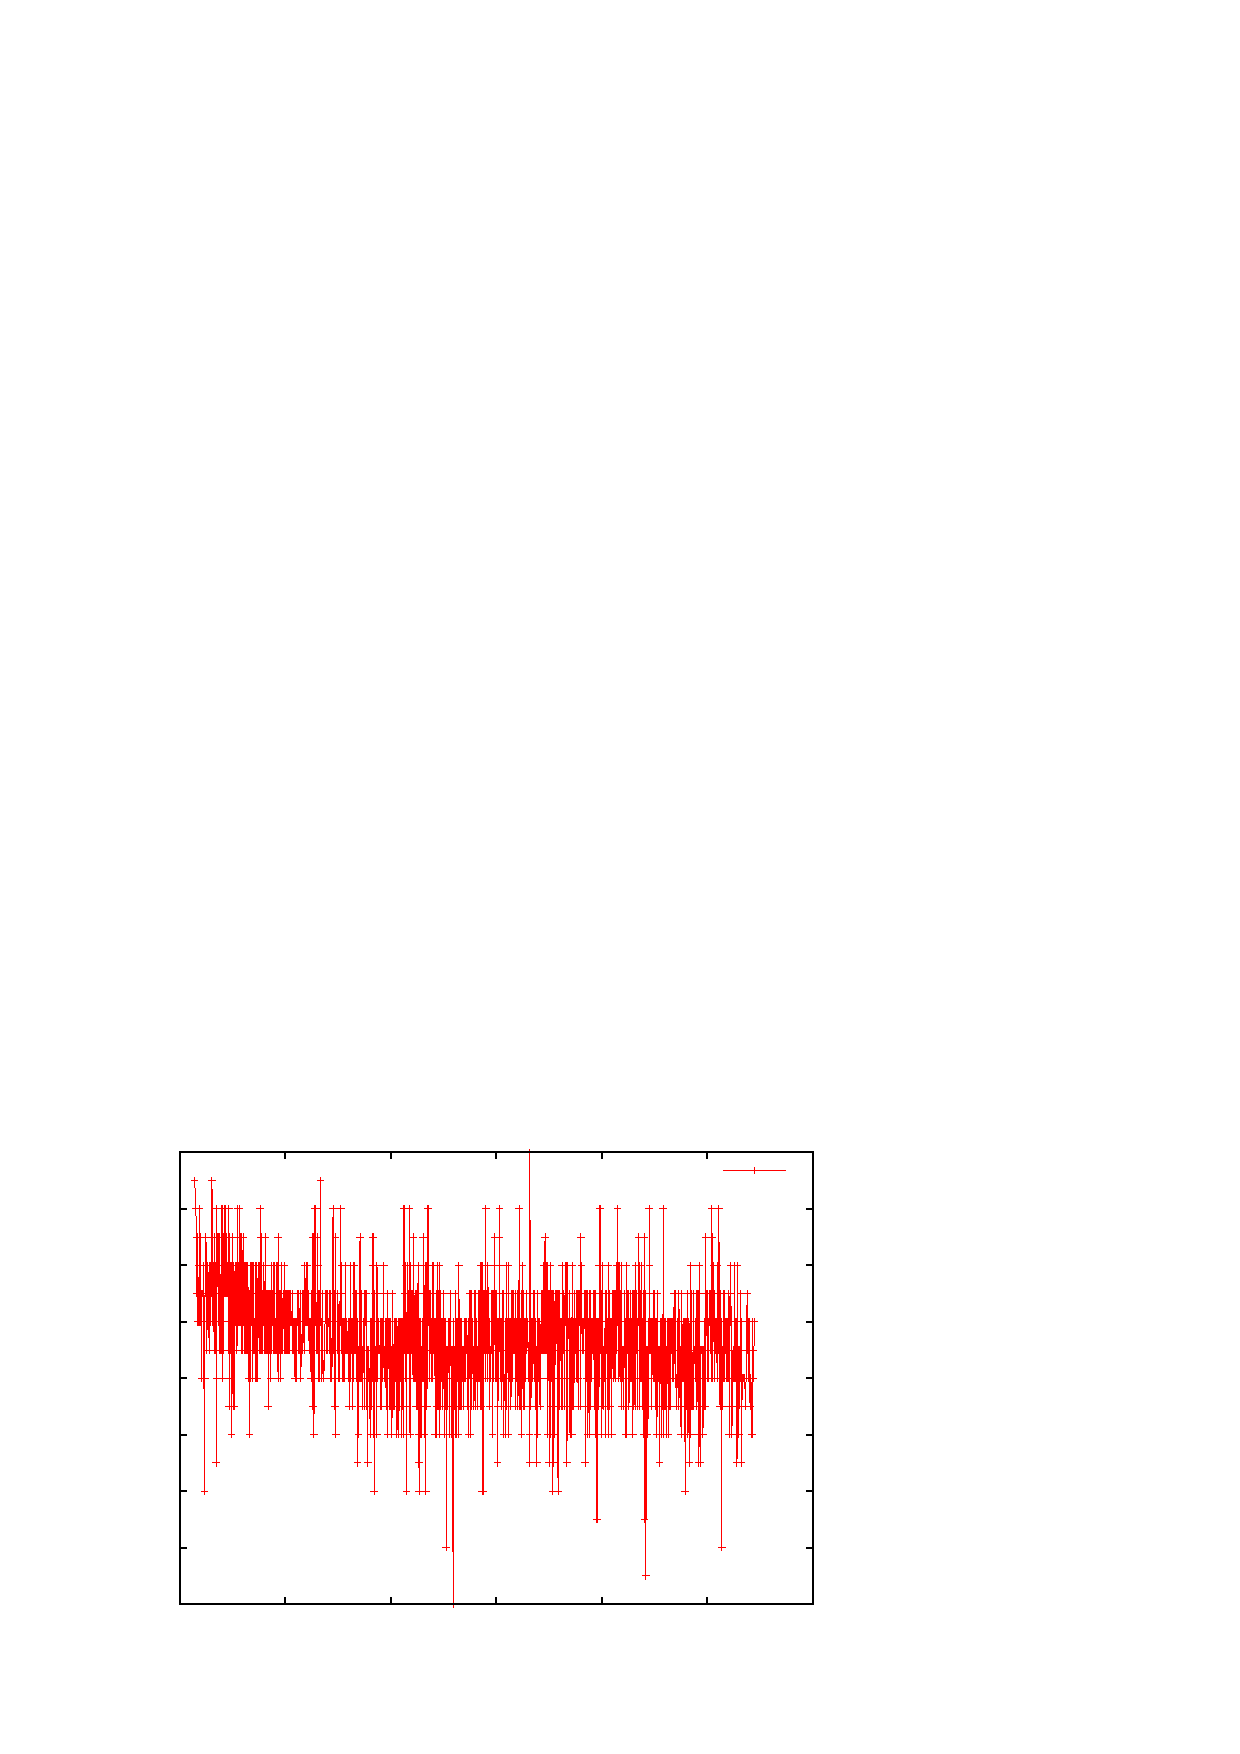
\includegraphics{figures/short_term_wifi.png}
    \caption{Variation of RSSI for closest AP. \label{fig:closestAPshortterm}}
\end{figure}


\subsection{During a thunderstorm}

Figure \ref{fig:closestAPthunderstorm} shows the variation of signal strength of
the closest AP for a smartphone placed in a room in NON-LOS configuration.

\begin{figure}\centering
    \includegraphics{figures/wifi_thunderstorm.png}
    \caption{Variation of RSSI for closest AP during a thunderstorm. \label{fig:closestAPthunderstorm}}
\end{figure}

\subsection{7 day study}

The Wifi AP RSSI values were monitored over a 7 day period (Jan 5 2011 - Jan 13 2011) from room S-152
and the resulting signal strength data was analyzed.

\begin{figure}\centering
    \includegraphics{figures/histogram_00_1C_F0_CB_EC_92.png}
    \caption{Distribution of RSSI values for the closest AP (00:1C:F0:CB:EC:92) \label{fig:histogram_00_1C_F0_CB_EC_92}}
\end{figure}

As you can see in Figure \ref{fig:histogram_00_1C_F0_CB_EC_92}, the signal strength
distribution is highly non-gaussian. This kind of distribution makes Kalman filters
unsuitable for use as the assumptions of gaussian (linear) distribution of 
input variables is unsatisfied.

\begin{figure}\centering
    \includegraphics{figures/histogram_00_1C_F0_CB_EC_95.png}
    \caption{Distribution of RSSI values for the AP near S-170 (00:1C:F0:CB:EC:95) \label{fig:histogram_00_1C_F0_CB_EC_95}}
\end{figure}

\begin{figure}\centering
    \includegraphics{figures/histogram_00_19_5B_77_A5_EE.png}
    \caption{Distribution of RSSI values for the AP near S-159 (00:19:5B:77:A5:EE) \label{fig:histogram_00_19_5B_77_A5_EE}}
\end{figure}

\begin{figure}\centering
    \includegraphics{figures/listplot_00_1C_F0_CB_EC_92.png}
    \caption{Point plot of RSSI values for the closest AP (00:1C:F0:CB:EC:92) \label{fig:listplot_00_1C_F0_CB_EC_92}}    
\end{figure}

\begin{figure}\centering
    \includegraphics{figures/moving_average.png}
    \caption{3 hour moving average of RSSI values}
\end{figure}

Figure \ref{fig:histogram_00_19_5B_77_A5_EE} doesn't show such a pronounced non-gaussian
nature whereas Figure \ref{fig:histogram_00_1C_F0_CB_EC_95} shows more leanings towards a
non-gaussian distribution.

Figure \ref{fig:listplot_00_1C_F0_CB_EC_92} is the time domain plot of the signal strength
samples. As you can see, the samples can be spread over a large domain even if the 
sample times differ by a couple of hours. Thus we can safely conclude that the 
input wifi signal is a highly noisy source of information.

\section{Effect of motion on signal strengths}

To analyze the effect of motion on the RSSI values from the APs, a simple walking
test was done along a corridoor. The variation of RSSI values seen from the APs in
the corridoor are shown in \ref{fig:wifi_corridoor_walk}.

\begin{figure}\centering
    \includegraphics{figures/wifi_corridoor_walk.png}
    \caption{RSSI values for APs during a corridoor walk \label{fig:wifi_corridoor_walk}}
\end{figure}

\todo{Improve figure with more APs and path description.}

\subsection{Inferences}
Effect of orientation with respect to AP is important. Signal strength values
even in LOS situations don't always behave nicely.

\section{Wifi Surveying}

A $1m \times 1m$ grid was set up on the ground and wifi readings were taken at 8
different orientations per point on the floor.

\todo{Describe the setup better.}

\begin{figure}
    \centering
    \includegraphics[width=5in,angle=270]{figures/grid_pic}
    \caption{Picture of the $1m \times 1m$ grid drawn on the floor}
\end{figure}

\section{Implementation of a KNN based positioning solution for KNN accuracy\label{sec:knn_pos}}

A KNN based location system was implemented to test location accuracy. 
This was work done as part of the project. Results are included here.

\begin{table}[h]
    \centering
    \caption{Performance of KNN based indoor positioning system \label{tab:knnperf}}
    \begin{tabular}{|l|c|c|c|}
    \hline
              & Mean Error $\bar{e}$ (m) & $\sigma_{error}$ (m) & $\bar{e} + 2 \sigma_{error}$ \\
    \hline
    \hline
    $K = 1$    & 2.8 & 2.7 & 8.2 \\
    $K = 2$    & 2.8 & 2.7 & 8.2 \\
    $K = 3$    & 2.7 & 2.7 & 8.1 \\
    $K = 4$    & 2.3 & 2.8 & 7.9 \\
    \hline
    \end{tabular}

\end{table}


\subsection{Improvements}
Use of SVM is likely to improve the accuracy further at room level. [Redpin]


\section{Dead Reckoning by direct integration: What doesn't work}
\section{What Doesn't work}
\todo{Fix this!}
Acceleration of the human body is too slow compared to gravity. Simple orientation changes produce high changes in acceleration along axes which are very difficult to filter out.
Numerical integration generates errors too quickly. With a high sampling rate, errors balloon.
Using the gyroscope for step detection (similar to foot mounted devices [insert reference]) – doesn’t work.


\section{Other issues}
Sensor noise, instability and bias. Effect of gravity and orientation on readings. Weather.



\chapter{Results\label{chap:results}}

\section{Hardware}
The hardware used to produce the results is the Samsung Nexus S (cobranded with
Google) running Android 2.3.4. The official specifications of the device can be
obtained from the manufacturer's website [link to website with reference] A
short listing of the sensors present on the device is given below based on how
the device reports the sensors via the software APIs:

\begin{enumerate}
\item KR3DM 3-axis Accelerometer
\item AK8973 3-axis Magnetic field sensor
\item AK8973 Orientation sensor
\item GP2A Light sensor
\item GP2A Proximity sensor
\item K3G Gyroscope sensor
\item Gravity Sensor
\item Linear Acceleration Sensor
\item Rotation Vector Sensor
\end{enumerate}

It may be noted that of these sensors, the Gravity sensor, the Linear
Acceleration Sensor and the Rotation Vector Sensor are derived sensors. They
depend on filtering the raw data sensed via the accelerometer and the
magnetometer to generate their sensed values. In essence, the Gravity sensor is
a low pass filter over the accelerometer values (since gravity is essentially
stable for the device at a particular orientation), the Linear Acceleration
Sensor is a high pass filter over the accelerometer values (the high frequency
changes in acceleration are presumed to occur due to device motion and thus
correspond to linear acceleration of the device) and the Rotation Vector Sensor
is a composite sensor that fuses Gravity information derived from the
3 axis Accelerometer and the magnetic field information derived from the
3 axis Magnetic field sensor to orient the device in the 3 Dimensional World 
Coordinate space. The actual method used to do so is described in the API
documentation \todo{Provide Reference}[reference to API documentation] and
further discussion is out of scope for this thesis.

\begin{figure}
\centering
    \includegraphics[height=3in]{figures/android_front}
    \includegraphics[height=3in]{figures/android_back}
\caption{Google Nexus S manufactured by Samsung}
\end{figure}

\section{Location Under Test}

The location chosen for performing all experimental verification of the
proposed work was Floor 3, Wing 6 and 7 of Ravindra Bhawan at the IIT Roorkee
campus. The environment is suitable for this purpose due to a number of reasons:

\begin{enumerate}
\item There are a large number of Wifi Access Points in close proximity 
    installed on the premises.
\item Wifi Access Points of neighbouring wings and floors provide diversity
    to the location fingerprints.
\item Long corridoors of around 30-32 metres each provide long stretches of
    similar environment for evaluation of algorithm performance over larger
    distances.
\end{enumerate}

A map of the location is shown in Figure \ref{fig:ravindra_map}. The red lines
indicate walls, blue lines indicate windows and green lines indicate doors.
Wifi Access Points are marked with stars on the map. This map has been used
for all the experiments detailed below.

\begin{figure}
    \centering
    \includegraphics[width=5in]{figures/ravindra_map.png}
    \caption{A map of the experimental environment\label{fig:ravindra_map}}
\end{figure}



\section{Step detection procedure}

Step detection for dead reckoning was done using accelerometer sensor data.
Two different methods were employed and the simple zero crossing method on 
unfiltered data was used as control to estimate the increase in accuracy of the
step detection procedure. A simple clamping technique was employed to filter the
raw acceleration as described in Section \ref{sec:NoiseClamping}.

The effect of the clamping on the raw accelerometer data is shown in 
Figure \ref{fig:accel_raw}. Figure \ref{fig:accel_diff} shows the sensor noise
that is rejected around zero enabling clean detection of peaks corresponding to
the steps.

The comparative graph of the performance of the step detection procedures 
is shown in Figure \ref{fig:csteps}. The correspondence to the ground truth
is shown in Table \ref{tbl:step_table}.

\begin{table}[tbph]
\centering
\begin{tabular}{||l|c||}
\hline
\hline
\textbf{Algorithm} & \textbf{Steps Detected} \\
\hline

Simple Zero Crossings Count & 109 \\
Zero Crossings on Filtered Data & 41 \\
Peaks and Valley Method & 41 \\
\textbf{Ground Truth} & \textbf{40} \\
\hline
\hline
\end{tabular}
\caption{Step Detection Performance\label{tbl:step_table}}
\end{table}

It can be seen that a simple Zero Crossing method performs similarly to the 
Peaks and Valley method. From the time based graph plotted in 
Figure \ref{fig:csteps}, it can be seen that the Peaks and Valley method 
slightly lags the Zero Crossing method in time. This is to be expected as this
method detects a step only when the next peak is detected and thus suffers a 
lag of about half a step.

\begin{figure}[tbph]
    \centering
    \includegraphics{figures/csteps.png}
    \caption{Performance of Step Detection Algorithms\label{fig:csteps}}
\end{figure}

\begin{figure}[tbph]
    \centering
    \includegraphics{figures/accel_raw.png}
    \caption{Performance of the Filtering algorithm \label{fig:accel_raw}}
\end{figure}

\begin{figure}[tbph]
    \centering
    \includegraphics{figures/accel_diff.png}
    \caption{Rejected signal from the Accelerometer sensor \label{fig:accel_diff}}
\end{figure}


\section{First Fix}

For any dead reckoning algorithm, it is important to provide a good starting
point. Low error in the starting location contributes to better
tracking performance.

In order to provide the starting point to the algorithm two approaches were
implemented:

\begin{enumerate}
\item Directly choose the starting location on a map using the capacitive 
    touchscreen
\item Select the starting location based on QRCode recognition using the onboard
    camera. The QRCodes were printed and pasted at specific locations 
    in the area under test.
\end{enumerate}

\missingfigure{QRCodes pasted on the wall}

\subsection{Experimental setup}

All the experments were performed with the same Android device (the Samsung 
Nexus S) and with the same application software. Users were familiar with 
touch screen phones and were well aware of the layout of the building. None of
the users had had any prior exposure to the map of the building and did not 
know the direction of True North. Details of the experiments performed 
are specified in Sections \ref{sec:direct_selection} and \ref{sec:qrcode_selection}

\subsection{Direct Selection of Location on a Map\label{sec:direct_selection}}

Five test subjects were asked to mark out their current position on a
map by simply touching the corresponding location on the map shown on the 
touchscreen of the device. The map was shown at a fixed resolution to all 
test subjects in order to make their responses comparable. 

The test were also allowed to retry locating themselves on the map in case they
were not satisfied with their initial results. All their location attempts were
logged for later analysis.The following facts were observed during the process of 
selection:

\begin{enumerate}
\item Users had an initial difficulty in orienting themselves with regard to 
    the map supplied.
\item As the map contained blocks of rooms that were similar looking, users
    made initial errors in orienting themselves. However, they attempted to 
    correct their errors when the mistake was realized.
\item Some users felt extremely frustrated by the direct selection procedure
    primarily because they could not mark out their locations precisely due
    to the large surface area of contact of their fingers with the touch
    screen. The variability of selection of the contact point while using 
    the touchscreen contributed to an increase in the number of attempts
    required to correctly mark their positions on the map.
\end{enumerate}

%\todo[inline]{Ask 5 people to select locations on a map and log data}
%\missingfigure{Table of error from true location}
%\missingfigure{Table of number of times attempted for satisfactory positioning}

\subsection{Camera based QRCode Method \label{sec:qrcode_selection}}

To evaluate the efficiency of determining first fix via QRCodes in comparison 
to the direct location selection method, an experiment was set up. 
The experiment was performed in conjunction with the experment of 
Section \ref{sec:direct_selection}, users were asked to locate themselves
by snapping a QRCode pasted on the wall instead of marking their starting 
location on a map.

The users were then positioned at various distances from the QRCode and 
asked whether they would make the effort to go to the QRCode to snap their
starting location while using the application or whether they would prefer
the manual method.

The following observations were made regarding the QRCode method for first
fix:

\begin{enumerate}
\item QRCode selection via the camera was a fast process, usually not requiring
    more than 10 seconds on behalf of the user.
\item Users were consistently located at distances less than 1 meter from 
    the QRCode. In most cases, the users were at a distance of around 30 cm 
    from the QRCode pasted on the wall. 
\item There was an instance where poor lighting delayed the capture of the
    QRCode and the QRCode could be successfully captured only after a 
    fluorescent tubelight was switched on to provide adequate lighting.
\end{enumerate}

\missingfigure{Image of a person snapping the QRCode with the camera}

\subsection{Comparison between the two methods}

After processing the results of the experiments, it was determined that 
users overwhelmingly preferred the QRCode method for first fix acquisition.
They were willing to walk up to $5 m$ to the nearest QRCoded location in 
order to take advantage of the facility.

\todo[inline]{Insert survey results}

\subsection{User Feedback}

Users in their comments indicated that potential improvements to the 
application were possible. For example, if the application could determine 
roughly their current location and then provide just that subset of the map
in which the user was located, the speed of providing the first fix location 
by a manual method could be improved.

\section{Determining the Training Constant}

In a separate experiment, three test subjects were asked to walk between 
2 QRCoded locations. The first fix was taken using the QRCode method and 
the training constant was thus estimated based on the number of steps 
detected and the known distance between the 2 QRCoded locations.

The locations used for this test were along a corridoor and were about $30 m$
apart. The tests were repeated thrice for each subject. The resulting 
step constants were taken as the average of the 3 runs.

\todo[inline]{Determining training constant}
\missingfigure{Table of training constant values}

\section{Step variation analysis}

To see the performance of the algorithm to step variations, an experiment 
was performed wherein a test subject walked at three distinct speeds
along a straight corridoor. The subject paused for a short while between 
the three distinct segments to maintain separation of speeds.

The three segments of the walk had the following
characteristics:

\begin{enumerate}
\item The test subject walked with very light steps, almost shuffling along. 
\item The test subject walked with regular steps along the corridoor.
\item The test subject walked with large steps along the corridoor in a motion
    that approximated running.
\end{enumerate}

The accelerometer graphs and the consequent step detections for this 
experiment are shown in Figure \ref{fig:step_variation}. The tabulated
results of the step detection process are shown in 
Table \ref{tbl:step_variation}. Note that the poor performance for 
shuffling steps is due to acceleration peaks not being sufficiently 
distinguishable from sensor noise and for the fast heavy steps is 
due to generation of spurious peaks while coming to an abrupt halt.
A smooth motion doesn't generate such issues and thus the step 
detection procedure is very accurate for that range.

\begin{table}[tbph]
    \centering
    \begin{tabular}{|l|c|c|}
        \hline
        \hline
        Step Segment & Actual Number of Steps & Steps Detected \\
        \hline
        Light Steps (Shuffle) & 10 & 5 \\
        Regular steps & 10 & 10 \\
        Fast (Heavy) steps & 15 & 18 \\
        \hline
        \hline
    \end{tabular}
    \caption{Step detections under step variations\label{tbl:step_variation}}
\end{table}

\begin{figure}
    \centering
    \includegraphics{figures/step_variation.png}
    \caption{Difference in step sizes and the corresponding variations in 
        step detection and step estimates\label{fig:step_variation}}
\end{figure}

\section{Test Paths\label{sec:test_paths}}

Five different test paths were used to test the performance of the system.
The features of these paths are described below. The paths themselves
are marked out in Figure \ref{fig:test_paths}.

\begin{enumerate}
\item Straight walk down a corridoor (A to B)
\item Straight walk down a corridoor, a U turn followed by a straight walk 
    to the starting point. (A to B and then B to A)
\item Zig-Zag walk down a corridoor (A to B).
\item A U shaped walk along all three corridoors. (A-B-C-D)
\item A U shaped walk along all three corridoors followed by a U turn and a 
    walk back to the starting location. (A-B-C-D-C-B-A)
\end{enumerate}

\begin{figure}
    \centering
    \includegraphics[width=5in]{figures/test_paths.jpg}
    \caption{Test paths for algorithm\label{fig:test_paths}}
\end{figure}


\section{Simple Dead Reckoning}

As discussed in the Literature Review (Chapter \ref{chap:literature_review}) and
in the Proposed Work (Chapter \ref{chap:proposed_method}), it is impossible to
directly obtain displacement information by double integration of the
accelerometer data. Hence, the step detection method was employed for tracking
the motion of the device as held by a walking human. The steps are integrated
with orientation information received from the magnetometer to create a 
simple dead reckoning system in accordance with the dynamical equation 
\eqref{eq:dr_eq}. The initial position for dead reckoning was obtained via
QRCodes in accordance with the description in Section \ref{sec:QRCodes}.


\subsection{Simple Dead Reckoning Results}

One of the well known weaknesses of the dead reckoning approach is that it
diverges quickly from the ground truth unless corrective measures are taken.
As a basic control for the results, a simple dead reckoning based 
tracking algorithm was developed. 

Figure \ref{fig:dr_path1} shows the quick divergence of the algorithm
from the expected path A-B. In fact, at the end of a simple straight walk of 
around $30 m$, the estimate for the location has diverged a lot from the 
actual location. It should also be noted that the path taken passes through
rooms and walls and thus, doesn't look like a natural path for the user.

Figure \ref{fig:dr_path5} shows the extreme divergence that takes place 
over long distances. Table \ref{tbl:dr_error_growth} chronicles the 
error growth that takes place for this path at the turning points of the path.
It is amply clear that Simple Dead Reckoning is not suitable for tracking
if implemented as-is.

\begin{table}[bph]
\centering
\begin{tabular}{l c c}
\hline
\hline
Location    & Distance Travelled    & Error \\
\hline
A           & 0                     & 0 \\
B           & 30 m                  & 3.761 m \\
C           & 56 m                  & 4.982 m \\
D           & 92 m                  & 5.416 m \\
\hline
\end{tabular}
\caption{Error growth over distance for Simple Dead Reckoning\label{tbl:dr_error_growth}}
\end{table}

\begin{figure}
    \centering
    \includegraphics[width=4in]{figures/dr_path1}
    \caption{Performance of Dead Reckoning for Test Path 1\label{fig:dr_path1}}
\end{figure}
 
\begin{figure}
    \centering
    \includegraphics[width=4in]{figures/dr_path5}
    \caption{Performance of Dead Reckoning for Test Path 5\label{fig:dr_path5}}
\end{figure}
 
 

\section{Reckoning with NN Wifi correction}

As per our groundwork described in Section \ref{sec:knn_pos} we know that the 
mean error for positioning using KNN is around $2.8 m$ with a standard deviation
that is nearly the same as the mean. Given the large errors incurred by 
the dead reckoning solution, we wish to analyze the performance of Dead 
Reckoning after Wifi data is integrated into the system.

\subsection{Wifi Survey}

We carried out a Wifi Survey of the test area and collected 1562 samples by 
carefully laying down a $1 m \times 1 m$ grid and collected samples. 8
different samples were collected per grid point at orientations that were
detected to be 45 degrees apart by the onboard magnetometer. By relying on
the magnetometer itself to specify orientation, the effect of local magnetic
fields was taken into account during the survey. However, sensor noise causes
the angle values actually recorded with the Wifi Signal Strength data to vary 
from the expected orientation of the user.

\subsection{Tracking Performance}

While implementing and testing out the implementation of the KNN based 
tracking solution, the resource and scaling limitations of the system 
came to fore. 

Because of it being a ``lazy" algorithm that consults the entire 
training dataset on every query for a position, the KNN algorithm
is computationally very intensive. Queries for obtaining a position based
on Wifi information was a slow process that even disrupted the UI of the 
application due to its heavy workload. Optimizations involving cacheing 
of data and short-circuiting the distance calculation step based on the 
orientation angle of the training sample viz a viz the current device 
orientation were implemented. With these optimizations, we were able 
to successfully run a hybrid Dead Reckoning system that utilized 
Wifi Access Point Received Signal Strengths and Step motion information
to track the device.

The performance of the algorithm was again judged based on the test paths 
mentioned in Section \ref{sec:test_paths}. Figure \ref{fig:nn_path1} shows
the track for Test path 1. A quick glance will indicate that the 
tracked endpoints are reasonably accurate (error < 2m), however, 
the subjective nature of the tracked path is very poor.

\begin{figure}
    \centering
    \includegraphics[width=5in]{figures/nn_path1}
    \caption{Performance of the KNN algorithm for Test Path 1\label{fig:nn_path1}}
\end{figure}

\begin{figure}
    \centering
    \includegraphics[width=5in]{figures/nn_path5}
    \caption{Performance of the KNN algorithm for Test Path 5\label{fig:nn_path5}}
\end{figure}


%\subsection{Case 2: Dead reckoning with KNN averaging}
%\subsection{Case 3: Dead reckoning with clamped wifi positioning}

\section{Reckoning with Integrated Map Information}

The results of the Wifi corrected reckoning as well as the data collected 
as part of the implementation of the KNN positioning system indicates that 
the location information utilizing Wifi data is very unstable. On the other
hand there is significant drift if we depend solely on the accelerometer
and the magnetometer to provide intertial tracking. In order to get 
better accuracy from the system, we require constant feedback from the 
environment. A way to achieve that is to use the fact that the device 
holder is always moving through ``passable" spaces on the map. Any motion
contrary to the allowed locations on the map would indicate tracking drift 
and a feedback loop would be set up to correct for such errors.

In this context, the particle filter's performance is analyzed with the
same test tracks as the other two algorithms. 

As can be seen amply in Figure \ref{fig:pf_path2} and Figure \ref{fig:pf_path4}
the tracking performance of this algorithm is excellent. The drift errors of the 
dead reckoning solution are compensated for by the map information
which ensures that only states consistent with the motion of the device 
are retained. Long term behaviour of the algorithm is also remarkably 
stable. Even after moving close to 100 m, the algorithm was able to 
maintain a tracking error of less than 1 m. This is illustrated in 
Figure \ref{fig:pf_path4}.


\begin{figure}
    \centering
    \includegraphics[width=5in]{figures/pf_path2}
    \caption{Performance of Reckoning with Map information for Test Path 2.\label{fig:pf_path2}}
\end{figure}

\begin{figure}
    \centering
    \includegraphics[width=5in]{figures/pf_path4}
    \caption{Performance of the Reckoning algorithm for Test Path 4.\label{fig:pf_path4}}
\end{figure}

%\subsection{Case 1: Probability of crossing walls is 0}
%\subsection{Case 2: Probability of crossing walls is finite}
%\todo[inline]{Should I even do it? It should come out with poorer results.}

%\subsection{Case 3: Resampling of impoverished data points with duplication}
%\subsection{Case 4: Resampling with introduction of Gaussian noise}
%\subsection{Case 4a: Use of averaged data points v/s random weighted data point}
%\subsection{Case 5: Accounting for bias in orientation sensor}
%\subsection{Case 6: Accounting for step size bias.}
%\subsection{Case 8: Simple heuristics to deal with impoverished samples}
%(retry, retry with greater inaccuracy, wifi)

\section{Comparison with published results}

With additional information at hand as well as suitable modifications to the 
dynamical equations of the system and care in avoiding particle degeneracy,
a significantly better accuracy has been achieved by this system as compared
to previous published works. 

The comparison of the 3 implemented methods can be done via the cumulative
distribution function which maps the percentage of sample points 
expected to be below a given error distance. 

\missingfigure{comparison table between results published and our methods}

\missingfigure{CDF of the errors of the methods (will take some time)}

\section{Summary of Results}
\todo[inline]{Which algorithms to pick based on the results, advantages and disadvantages}

The complete set of results are stated in the appendix as they were too 
voluminous to state in the main body of the report.

\section{Issues faced}
Incorrect step sizes yielded states in which no further progress was possible
using data from the inertial sensors. Hence we had to resort to wifi data to get
out of the blind spot.

Limited processing power and near-realtime time constraints of operation
constrain computational complexity of the solution.

Surveying is the biggest issue in this system.

Computational complexity and scaling issues.

\begin{figure}
    \centering
    \includegraphics[width=5in]{figures/pf_bad.png}
    \caption{Sometimes, the recovery process leads to a sequence of states 
        which is equivalent to getting lost.\label{fig:pf_bad}}
\end{figure}


\chapter{Summary and Future Work\label{chap:summary}}

\section{Summary of the Work}

As per the problem statement described in Section \ref{sec:problem_description},
an indoor tracking solution based on a particle filter approach for pedestrians
has been developed for the Android smartphone. The performance of the algorithm 
has been evaluated and it has shown an improvement against prior work in the 
area.

Based on the insights gained during this work, a few points need to be stated
in conclusion:

\begin{enumerate}
\item QRCodes are excellent tools for providing first fixes to tracking algorithms. They are reasonably scalable
    and extremely easy to use.
\item Wifi is a poor choice of signal source to correct for drift errors for step estimate based tracking solutions. This is because Wifi signal sources are too noisy that they are only able to correct gross drift errors. In fact, using Wifi data for drift correction probably degrades accuracy rather than improves it. 
\item Having a Wifi survey of an area is a very time consuming matter. However, it provides an additional way to resolve situtations where the particle filter gets lost. 
\item Treating all particles at par (as is done in this algorithm) reduces computational complexity of the particle filter by eliminating the reweighting done at each step.
\item It is very important to analyze the parameters of the sensors to choose appropriate values for the algorithm. Doing so ensures particle conservation and thus reduces the computational load on the system.
\end{enumerate}

The system has shown excellent performance in the tests and as an outcome of this thesis, it is recommended that only map information be used for drift correction instead of a combination of Map information and Wifi data. 

Of course, as no system is perfect, this system too has its shortcomings and limitations: 

\begin{enumerate}
\item Due to the lower number of particles allowed, the algorithm has a higher tendency to get lost.
\item Once lost, it is hard to recover and recovery is usually associated with some tracking error.
\item The system requires a Wifi Survey of the test area for error recovery which is time consuming and non-scalable. This may be avoided however if we are willing to sacrifice a better chance at recovery in case the algorithm gets lost.
\item Using the lazy Nearest Neighbour algorithm is expensive in time and memory consumption and is not very scalable.
\item Small steps cannot be detected due to limitations of the step detection algorithm.
\item Maps with large open spaces provide very little feedback to the tracking algorithm and thus the tracking quality degrades.
\end{enumerate}

All these points provide scope for future work on this system.

%\begin{figure}
%    \centering
%    \includegraphics[width=5in]{figures/pf_bad.png}
%    \caption{Sometimes, the recovery process leads to a sequence of states 
%        which is equivalent to getting lost.\label{fig:pf_bad}}
%\end{figure}


\section{Limitations}

The one thing that this algorithm is unable to take into account is when a user decides to move backwards
while retaining the same direction of the smartphone. 
Since the algorithm makes an assumption of forward motion only, moving backwards significantly affects the accuracy of the tracking algorithm and the algorithm quickly gets lost. This is a limitation of the system.


\section{Future enhancements}

There is a lot of scope for improving a number of aspects of the 
algorithms proposed. For example, we need to look at improving $MapSelect$,
integrating information from barometric sensors as and when they are made
available on handheld devices. We also need to figure out how to modify
the information to be put into first fix QRCodes to link up maps of 
the same building. SVM can also be used to increase the accuracy of the 
recovered position on the lines of the work done by \cite{ETHLuba} for 
Redpin\cite{Redpin}.

On the implementation front, performance of the solution, though 
adequate, can be significantly improved to enable a greater number of particles
to be evolved. For example, 
improvements can be achieved by leveraging thread parallelism and a 
producer consumer model to allow for higher system lag in the case of 
a recovery event. The UI can be made event driven from the current 
polling model to increase responsiveness. Also, the Android NDK can be used 
to write the performance intensive parts of the solution in C.


\section{Crowdsourcing a Signal Strength Map}

An application of this thesis that arises naturally from the results is that
the base algorithm can be used to set up a crowdsourcing system that will 
eventually generate a Wifi signal strength map of a large test area based 
solely on user inputs generated while they are using the tracking application. 
This would be beneficial for bootstrapping projects like \cite{Redpin} for 
providing lower complexity solutions to the indoor positioning problem. 
This aspect requires greater thought and research.






\appendix

%\todo[inline]{Enable this appendix later}
\chapter{Test results for all algorithms}

\section{Simple Dead Reckoning}

Figures \ref{fig:sdr_path1}, \ref{fig:sdr_path2}, \ref{fig:sdr_path3}, \ref{fig:sdr_path4}, \ref{fig:sdr_path5}
show the results of simple dead reckoning on the Test Paths 1-5.

\begin{figure}
    \centering
    \includegraphics[width=3in]{figures/sdr_path1}
    \caption{Simple Dead Reckoning Path 1\label{fig:sdr_path1}}
\end{figure}

\begin{figure}
    \centering
    \includegraphics[width=3in]{figures/sdr_path2}
    \caption{Simple Dead Reckoning Path 2\label{fig:sdr_path2}}
\end{figure}

\begin{figure}
    \centering
    \includegraphics[width=3in]{figures/sdr_path3}
    \caption{Simple Dead Reckoning Path 3\label{fig:sdr_path3}}
\end{figure}

\begin{figure}
    \centering
    \includegraphics[width=3in]{figures/sdr_path4}
    \caption{Simple Dead Reckoning Path 4\label{fig:sdr_path4}}
\end{figure}

\begin{figure}
    \centering
    \includegraphics[width=3in]{figures/sdr_path5}
    \caption{Simple Dead Reckoning Path 5\label{fig:sdr_path5}}
\end{figure}

\section{Wifi Corrected Reckoning}

Figures \ref{fig:wcr_path1}, \ref{fig:wcr_path2}, \ref{fig:wcr_path3}, \ref{fig:wcr_path4}, \ref{fig:wcr_path5}
show the results of Wifi corrected reckoning on the Test Paths 1-5.


\begin{figure}
    \centering
    \includegraphics[width=3in]{figures/wcr_path1}
    \caption{Wifi Corrected Reckoning Path 1\label{fig:wcr_path1}}
\end{figure}

\begin{figure}
    \centering
    \includegraphics[width=3in]{figures/wcr_path2}
    \caption{Wifi Corrected Reckoning Path 2\label{fig:wcr_path2}}
\end{figure}

\begin{figure}
    \centering
    \includegraphics[width=3in]{figures/wcr_path3}
    \caption{Wifi Corrected Reckoning Path 3\label{fig:wcr_path3}}
\end{figure}

\begin{figure}
    \centering
    \includegraphics[width=3in]{figures/wcr_path4}
    \caption{Wifi Corrected Reckoning Path 4\label{fig:wcr_path4}}
\end{figure}

\begin{figure}
    \centering
    \includegraphics[width=3in]{figures/wcr_path5}
    \caption{Wifi Corrected Reckoning Path 5\label{fig:wcr_path5}}
\end{figure}


\section{Reckoning with Map Information}

Figures \ref{fig:mcr_path1}, \ref{fig:mcr_path2}, \ref{fig:mcr_path3}, \ref{fig:mcr_path4}, \ref{fig:mcr_path5}
show the results of particle filtered reckoning with map information on the Test Paths 1-5.


\begin{figure}
    \centering
    \includegraphics[width=3in]{figures/mcr_path1}
    \caption{Reckoning with Map Information Path 1\label{fig:mcr_path1}}
\end{figure}

\begin{figure}
    \centering
    \includegraphics[width=3in]{figures/mcr_path2}
    \caption{Reckoning with Map Information Path 2\label{fig:mcr_path2}}
\end{figure}

\begin{figure}
    \centering
    \includegraphics[width=3in]{figures/mcr_path3}
    \caption{Reckoning with Map Information Path 3\label{fig:mcr_path3}}
\end{figure}

\begin{figure}
    \centering
    \includegraphics[width=3in]{figures/mcr_path4}
    \caption{Reckoning with Map Information Path 4\label{fig:mcr_path4}}
\end{figure}

\begin{figure}
    \centering
    \includegraphics[width=3in]{figures/mcr_path5}
    \caption{Reckoning with Map Information Path 5\label{fig:mcr_path5}}
\end{figure}



%\input{appendix-survey_form.tex}

\backmatter

\singlespace
\bibliographystyle{IEEEtran}
\addcontentsline{toc}{chapter}{Bibliography}
\bibliography{IEEEfull,mybib}


\end{document}
